\section{Abbildungen: $\mathbb{R} \rightarrow \mathbb{R}^n$}

\subsection{Linearisierung}
$f(t+\Delta t) \approx f(t) + \Delta t \cdot f'(t)$

\subsection{Tangentenvektor}
\begin{itemize}
	\item Gleichung: \\
	\begin{displaymath}
		f(t) =
		\begin{pmatrix}
			x(t) \\ y(t) \\ z(t)
		\end{pmatrix}
		\Rightarrow
		f'(t) =
		\begin{pmatrix}
			\dot{x}(t) \\ \dot{y}(t) \\ \dot{z}(t)
		\end{pmatrix}
	\end{displaymath}
\end{itemize}

\subsection{Parameterdarstellung}
\begin{itemize}
	\item Beispiel für Parameterdarstellung k von f mit Parameter t:
	\begin{displaymath}
		f(\theta) =
		\begin{pmatrix}
			x(\theta) \\ y(\theta) \\ z(\theta)
		\end{pmatrix}
		\Rightarrow
		k(\theta) =
		\begin{pmatrix}
			x(t(\theta)) \\ y(t(\theta)) \\ z(t(\theta))
		\end{pmatrix}
	\end{displaymath}
	\begin{itemize}
		\item Definitionsbereich neu berechnen
		\item Darstellung nur ohne weiteres möglich, wenn monoton
	\end{itemize}
	\item Ableitung: \\
	$|f'(t)| = \sqrt{\dot{x}(t)^2 + \dot{y}(t)^2 + \dot{z}(t)^2}$
	\item Integral: \\
	$\int_a^b |f'(t)| ds$
\end{itemize}

\subsection{Bogenlänge}
\begin{itemize}
	\item Normale Funktionen: $L_{a,b} \approx \int_a^b \sqrt{1+f'(x)^2} dx$
	\item Parameterdarstellung:
	$L_{a,b} = \int_a^b |f'(t)| ds$
	\begin{itemize}
		\item Bogenlänge Schraubenlinie:
		$L_{a,b} = \int_a^b (\sqrt{R^2 + v^2}\cdot \alpha ) d\alpha$
		\item Bogenlänge Zykloide:
		$L_{a,b} = \int_a^b (2 R\cdot sin(\frac{\varphi}{2})) d\varphi$
		\item Bogenlänge bei Archimedische Spirale:
		$L_{a,b} = \int_a^b \sqrt{r'(\varphi)^2 + r(\varphi)^2} d\varphi$
	\end{itemize}
\end{itemize}

\subsection{Krümmung}
\begin{itemize}
	\item Normale Funktionen: $K(x) = \frac{f''(x)}{\sqrt{1+f'(x)^2}^3}$
	\item Parametrisiert:
	$K(t) = \frac
		{\ddot{y} \dot{x} - \dot{y} \ddot{x}}
		{\big ( \dot{x} \sqrt{1 + \frac{ \dot{y} }{ \dot{x} }^2} \big )^3}
	$
	\item Krümmungskreis Radius: $\frac{1}{K(x)}$ \\
	\begin{figure}[h!]
		\centering
		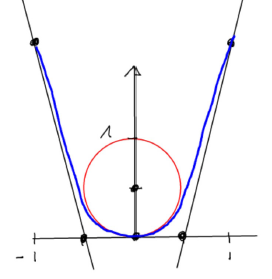
\includegraphics[scale=.5]{pics/kruemmungskreis}
		\caption{Krümmunkskreis im Scheitelpunkt}
	\end{figure}
\end{itemize}

\pagebreak

\subsection{Linienintegrale}
\subsubsection{1. Art:}
\begin{itemize}
	\item Parameterdarstellung $K: \mathbb{R} \rightarrow \mathbb{R}^n$
	\item Funktion $F: \mathbb{R}^n \rightarrow \mathbb{R}$
\end{itemize}
$\Rightarrow \int_a^b F(K(t)) \cdot |K'(t)| dt$

\subsubsection{2. Art:}
